\documentclass[12pt,t]{beamer}
\usepackage{graphicx}
\setbeameroption{hide notes}
\setbeamertemplate{note page}[plain]

% get rid of junk
\usetheme{default}
\beamertemplatenavigationsymbolsempty
\hypersetup{pdfpagemode=UseNone} % don't show bookmarks on initial view

% font
\usepackage{fontspec}
\setsansfont{TeX Gyre Heros}
\setbeamerfont{note page}{family*=pplx,size=\footnotesize} % Palatino for notes
% "TeX Gyre Heros can be used as a replacement for Helvetica"
% In Unix, unzip the following into ~/.fonts
% In Mac, unzip it, double-click the .otf files, and install using "FontBook"
%   http://www.gust.org.pl/projects/e-foundry/tex-gyre/heros/qhv2.004otf.zip

% named colors
\definecolor{offwhite}{RGB}{249,242,215}
% \definecolor{foreground}{RGB}{255,255,255}
\definecolor{foreground}{RGB}{0,0,0}
% \definecolor{background}{RGB}{24,24,24}
\definecolor{background}{RGB}{255,255,255}
\definecolor{title}{RGB}{107,174,214}
\definecolor{gray}{RGB}{100,100,100}
\definecolor{subtitle}{RGB}{102,255,204}
\definecolor{hilight}{RGB}{20,180,204}
\definecolor{vhilight}{RGB}{255,111,207}
\definecolor{lolight}{RGB}{155,155,155}
%\definecolor{green}{RGB}{125,250,125}

% use those colors
\setbeamercolor{titlelike}{fg=title}
\setbeamercolor{subtitle}{fg=subtitle}
\setbeamercolor{institute}{fg=gray}
\setbeamercolor{normal text}{fg=foreground,bg=background}
\setbeamercolor{item}{fg=foreground} % color of bullets
\setbeamercolor{subitem}{fg=gray}
\setbeamercolor{itemize/enumerate subbody}{fg=gray}
\setbeamertemplate{itemize subitem}{{\textendash}}
\setbeamerfont{itemize/enumerate subbody}{size=\footnotesize}
\setbeamerfont{itemize/enumerate subitem}{size=\footnotesize}

% page number
\setbeamertemplate{footline}{%
    \raisebox{5pt}{\makebox[\paperwidth]{\hfill\makebox[20pt]{\color{gray}
          \scriptsize\insertframenumber}}}\hspace*{5pt}}

% add a bit of space at the top of the notes page
\addtobeamertemplate{note page}{\setlength{\parskip}{12pt}}

% a few macros
\newcommand{\bi}{\begin{itemize}}
\newcommand{\ei}{\end{itemize}}
\newcommand{\ig}{\includegraphics}
\newcommand{\subt}[1]{{\footnotesize \color{subtitle} {#1}}}


% title info
\title{Data structures II}
% \subtitle{Theory, Representation, and Algorithms}
\author{Gregor Behnke}
\institute{Institute of Artificial Intelligence\\ Ulm University}
\date{\tiny based on Bjarki Ágúst Guðmundsson's and Tómas Ken Magnússon's\\Competitive Programming}
% \date{\href{http://www.biostat.wisc.edu/~kbroman}{\tt \scriptsize biostat.wisc.edu/{\textasciitilde}kbroman}
% \\[-4pt]
% \href{http://github.com/kbroman}{\tt \scriptsize github.com/kbroman}
% }

% Tikz
\usepackage{tikz}
\usetikzlibrary{arrows,shapes,matrix,calc}
\pgfdeclarelayer{bg}    % declare background layer
\pgfsetlayers{bg,main}

% Minted
\usepackage{minted}
\usemintedstyle{tango}
\newminted{cpp}{fontsize=\footnotesize}

% Graph styles
\tikzstyle{vertex}=[circle,fill=black!50,minimum size=15pt,inner sep=0pt, font=\small]
\tikzstyle{selected vertex} = [vertex, thick, draw=vhilight, fill=vhilight!50]
\tikzstyle{edge} = [draw,thick,-]
\tikzstyle{dedge} = [draw,thick,->]
\tikzstyle{weight} = [font=\scriptsize,pos=0.5]
\tikzstyle{selected edge} = [draw,line width=2pt,-,red!50]
\tikzstyle{ignored edge} = [draw,line width=5pt,-,black!20]


\begin{document}

% title slide
{
    \setbeamertemplate{footline}{} % no page number here
    \frame{
        \titlepage
    }
}


\begin{frame}{Today we're going to cover}
    \vspace{40pt}
    \bi
        \item Study range queries
        \item Learn about Segment Trees
        \item Learn about Fenwick Trees
    \ei
\end{frame}


% TODO: Range queries on a dynamic array
\begin{frame}{Range sum on a dynamic array}
    \bi
        \item What if we want to support:
            \bi
                \item sum over a range
                \item updating an element
            \ei
    \ei

    \begin{center}
        \begin{tabular}{|c|c|c|c|c|c|c|}
            \hline
            \color<2,3,6,7>{vhilight}{1} & \color<2,3,6,7>{vhilight}{0} & \color<2,3,6,7>{vhilight}{7} & \color<2,3,4,5,6,7>{vhilight}{\only<-4>{8}\only<5->{-2}} & \color<2,3,6,7>{vhilight}{5} & \color<2,3,6,7>{vhilight}{9} & \color<2,3,6,7>{vhilight}{3} \\
            \hline
        \end{tabular}
    \end{center}

    \bi
        \onslide<2->{\item $\mathrm{sum}(0,6)\onslide<3->{ = 33}$}
        \onslide<4->{\item $\mathrm{update}(3,-2)$}
        \onslide<6->{\item $\mathrm{sum}(0,6)\onslide<7->{ = 23}$}
        \vspace{20pt}
        \onslide<8->{\item How do we support these queries efficiently?}
    \ei
\end{frame}

\begin{frame}[fragile]{Segment Tree}
            \begin{figure}
                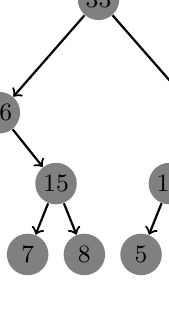
\begin{tikzpicture}[scale=1.8,auto,swap]
                    \onslide<2->{
                        \node[vertex] (0) at (-0.8,0.2) {1};
                        \node[vertex] (1) at (-0.4,0.2) {0};
                        \node[vertex] (2) at (0.0,0.2) {7};
                        \node[vertex] (3) at (0.4,0.2) {8};
                        \node[vertex] (4) at (0.8,0.2) {5};
                        \node[vertex] (5) at (1.2,0.2) {9};
                        \node[vertex] (6) at (1.6,0.2) {3};
                    }

                    \onslide<3->{
                        \node[vertex] (7) at (-0.6,0.7) {1};
                        \node[vertex] (8) at (0.2,0.7) {15};
                        \node[vertex] (9) at (1.0,0.7) {14};
                    }

                    \onslide<4->{
                        \node[vertex] (10) at (-0.2,1.2) {16};
                        \node[vertex] (11) at (1.2,1.2) {17};
                    }

                    \onslide<5->{
                        \node[vertex] (12) at (0.5,2.0) {33};
                    }

                    \onslide<3->{
                        \path[dedge] (7) -- (0);
                        \path[dedge] (7) -- (1);
                        \path[dedge] (8) -- (2);
                        \path[dedge] (8) -- (3);
                        \path[dedge] (9) -- (4);
                        \path[dedge] (9) -- (5);
                    }

                    \onslide<4->{
                        \path[dedge] (10) -- (7);
                        \path[dedge] (10) -- (8);
                        \path[dedge] (11) -- (9);
                        \path[dedge] (11) -- (6);
                    }

                    \onslide<5->{
                        \path[dedge] (12) -- (10);
                        \path[dedge] (12) -- (11);
                    }

                    \pgfresetboundingbox
                    \path [use as bounding box] (0,0) rectangle (0.8,1.8);
                \end{tikzpicture}
            \end{figure}

    \begin{center}
        \begin{tabular}{|c|c|c|c|c|c|c|}
            \hline
                1 & 0 & 7 & 8 & 5 & 9 & 3 \\
            \hline
        \end{tabular}
    \end{center}

    \bi
        \onslide<6>{\item Each vertex contains the sum of some segment of the array}
    \ei
\end{frame}

\begin{frame}[fragile]{Segment Tree - Code}
    \begin{minted}[fontsize=\scriptsize]{cpp}
struct segment_tree {
    segment_tree *left, *right;
    int from, to, value;
    segment_tree(int from, int to)
        : from(from), to(to), left(NULL), right(NULL), value(0) { }
};

segment_tree* build(const vector<int> &arr, int l, int r) {
    if (l > r) return NULL;
    segment_tree *res = new segment_tree(l, r);
    if (l == r) {
        res->value = arr[l];
    } else {
        int m = (l + r) / 2;
        res->left = build(arr, l, m);
        res->right = build(arr, m + 1, r);
        if (res->left != NULL) res->value += res->left->value;
        if (res->right != NULL) res->value += res->right->value;
    }
    return res;
}
    \end{minted}
\end{frame}

\begin{frame}[fragile]{Querying a Segment Tree}
            \begin{figure}
                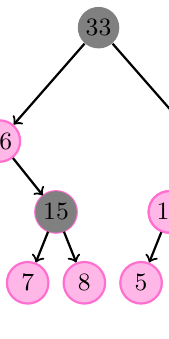
\begin{tikzpicture}[scale=1.8,auto,swap]

                    \onslide<-2,4->{
                        \node[vertex] (0) at (-0.8,0.2) {1};
                        \node[vertex] (1) at (-0.4,0.2) {0};
                        \node[vertex] (2) at (0.0,0.2) {7};
                        \node[vertex] (3) at (0.4,0.2) {8};
                        \node[vertex] (4) at (0.8,0.2) {5};
                        \node[vertex] (5) at (1.2,0.2) {9};
                    }
                    \onslide<3>{
                        \node[selected vertex] (0) at (-0.8,0.2) {1};
                        \node[selected vertex] (1) at (-0.4,0.2) {0};
                        \node[selected vertex] (2) at (0.0,0.2) {7};
                        \node[selected vertex] (3) at (0.4,0.2) {8};
                        \node[selected vertex] (4) at (0.8,0.2) {5};
                        \node[selected vertex] (5) at (1.2,0.2) {9};
                    }
                    \node[vertex] (6) at (1.6,0.2) {3};

                    \onslide<-3>{
                        \node[vertex] (7) at (-0.6,0.7) {1};
                        \node[vertex] (8) at (0.2,0.7) {15};
                        \node[vertex] (9) at (1.0,0.7) {14};
                    }
                    \onslide<4>{
                        \node[selected vertex] (7) at (-0.6,0.7) {1};
                        \node[selected vertex] (8) at (0.2,0.7) {15};
                        \node[selected vertex] (9) at (1.0,0.7) {14};
                    }
                    \onslide<5->{
                        \node[vertex] (7) at (-0.6,0.7) {1};
                        \node[vertex] (8) at (0.2,0.7) {15};
                        \node[selected vertex] (9) at (1.0,0.7) {14};
                    }

                    \onslide<-5>{
                        \node[vertex] (10) at (-0.2,1.2) {16};
                    }
                    \onslide<5->{
                        \node[selected vertex] (10) at (-0.2,1.2) {16};
                    }
                    \node[vertex] (11) at (1.2,1.2) {17};

                    \node[vertex] (12) at (0.5,2.0) {33};

                    \path[dedge] (7) -- (0);
                    \path[dedge] (7) -- (1);
                    \path[dedge] (8) -- (2);
                    \path[dedge] (8) -- (3);
                    \path[dedge] (9) -- (4);
                    \path[dedge] (9) -- (5);

                    \path[dedge] (10) -- (7);
                    \path[dedge] (10) -- (8);
                    \path[dedge] (11) -- (9);
                    \path[dedge] (11) -- (6);

                    \path[dedge] (12) -- (10);
                    \path[dedge] (12) -- (11);

                    \pgfresetboundingbox
                    \path [use as bounding box] (0,0) rectangle (0.8,2.0);
                \end{tikzpicture}
            \end{figure}

    \begin{center}
        \begin{tabular}{|c|c|c|c|c|c|c|}
            \hline
            \color<2->{vhilight}{1} & \color<2->{vhilight}{0} & \color<2->{vhilight}{7} & \color<2->{vhilight}{8} & \color<2->{vhilight}{5} & \color<2->{vhilight}{9} & 3 \\
            \hline
        \end{tabular}
    \end{center}

    \bi
        % \item How do we query the tree?
        \onslide<2->{\item $\mathrm{sum}(0,5)\onslide<6->{= 16 + 14 = 30}$}
        \onslide<7->{\item We only need to consider a few vertices to get the entire range}
        \onslide<8->{\item But how do we find them?}
    \ei
\end{frame}

\begin{frame}[fragile]{Querying a Segment Tree}
            \begin{figure}
                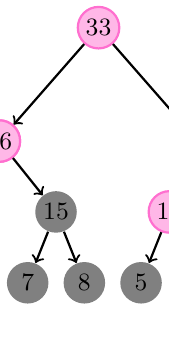
\begin{tikzpicture}[scale=1.8,auto,swap]

                    % \onslide<-2,4->{
                        \node[vertex] (0) at (-0.8,0.2) {1};
                        \node[vertex] (1) at (-0.4,0.2) {0};
                        \node[vertex] (2) at (0.0,0.2) {7};
                        \node[vertex] (3) at (0.4,0.2) {8};
                        \node[vertex] (4) at (0.8,0.2) {5};
                        \node[vertex] (5) at (1.2,0.2) {9};
                    % }
                    % \onslide<3>{
                    %     \node[selected vertex] (0) at (-0.8,0.2) {1};
                    %     \node[selected vertex] (1) at (-0.4,0.2) {0};
                    %     \node[selected vertex] (2) at (0.0,0.2) {7};
                    %     \node[selected vertex] (3) at (0.4,0.2) {8};
                    %     \node[selected vertex] (4) at (0.8,0.2) {5};
                    %     \node[selected vertex] (5) at (1.2,0.2) {9};
                    % }
                    \onslide<-4,6->{
                        \node[vertex] (6) at (1.6,0.2) {3};
                    }
                    \onslide<5>{
                        \node[selected vertex] (6) at (1.6,0.2) {3};
                    }

                    % \onslide<-3>{
                        \node[vertex] (7) at (-0.6,0.7) {1};
                        \node[vertex] (8) at (0.2,0.7) {15};
                    \onslide<-4>{
                        \node[vertex] (9) at (1.0,0.7) {14};
                    }
                    \onslide<5->{
                        \node[selected vertex] (9) at (1.0,0.7) {14};
                    }
                    % }
                    % \onslide<4>{
                    %     \node[selected vertex] (7) at (-0.6,0.7) {1};
                    %     \node[selected vertex] (8) at (0.2,0.7) {15};
                    %     \node[selected vertex] (9) at (1.0,0.7) {14};
                    % }
                    % \onslide<5->{
                    %     \node[vertex] (7) at (-0.6,0.7) {1};
                    %     \node[vertex] (8) at (0.2,0.7) {15};
                    %     \node[selected vertex] (9) at (1.0,0.7) {14};
                    % }

                    \onslide<-3>{
                        \node[vertex] (10) at (-0.2,1.2) {16};
                        \node[vertex] (11) at (1.2,1.2) {17};
                    }
                    \onslide<4>{
                        \node[selected vertex] (10) at (-0.2,1.2) {16};
                        \node[selected vertex] (11) at (1.2,1.2) {17};
                    }
                    \onslide<5->{
                        \node[selected vertex] (10) at (-0.2,1.2) {16};
                        \node[vertex] (11) at (1.2,1.2) {17};
                    }

                    \onslide<-2,4->{
                        \node[vertex] (12) at (0.5,2.0) {33};
                    }
                    \onslide<3>{
                        \node[selected vertex] (12) at (0.5,2.0) {33};
                    }

                    \path[dedge] (7) -- (0);
                    \path[dedge] (7) -- (1);
                    \path[dedge] (8) -- (2);
                    \path[dedge] (8) -- (3);
                    \path[dedge] (9) -- (4);
                    \path[dedge] (9) -- (5);

                    \path[dedge] (10) -- (7);
                    \path[dedge] (10) -- (8);
                    \path[dedge] (11) -- (9);
                    \path[dedge] (11) -- (6);

                    \path[dedge] (12) -- (10);
                    \path[dedge] (12) -- (11);

                    \pgfresetboundingbox
                    \path [use as bounding box] (0,0) rectangle (0.8,2.0);
                \end{tikzpicture}
            \end{figure}

    \begin{center}
        \begin{tabular}{|c|c|c|c|c|c|c|}
            \hline
            \color<2->{vhilight}{1} & \color<2->{vhilight}{0} & \color<2->{vhilight}{7} & \color<2->{vhilight}{8} & \color<2->{vhilight}{5} & \color<2->{vhilight}{9} & 3 \\
            \hline
        \end{tabular}
    \end{center}

    \bi
        \item $\mathrm{sum}(0,5)$
    \ei
\end{frame}

\begin{frame}[fragile]{Querying a Segment Tree - Code}
    \vspace{50pt}
    \begin{minted}[fontsize=\scriptsize]{cpp}
int query(segment_tree *tree, int l, int r) {
    if (tree == NULL) return 0;
    if (l <= tree->from && tree->to <= r) return tree->value;
    if (tree->to < l) return 0;
    if (r < tree->from) return 0;
    return query(tree->left, l, r) + query(tree->right, l, r);
}
    \end{minted}
\end{frame}


\begin{frame}[fragile]{Updating a Segment Tree}
    \begin{figure}
        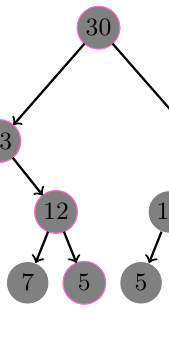
\begin{tikzpicture}[scale=1.8,auto,swap]
            \node[vertex] (0) at (-0.8,0.2) {1};
            \node[vertex] (1) at (-0.4,0.2) {0};
            \node[vertex] (2) at (0.0,0.2) {7};
            \onslide<-2>{
                \node[vertex] (3) at (0.4,0.2) {8};
            }
            \onslide<3>{
                \node[selected vertex] (3) at (0.4,0.2) {8};
            }
            \onslide<4>{
                \node[selected vertex] (3) at (0.4,0.2) {5};
            }
            \onslide<5->{
                \node[vertex] (3) at (0.4,0.2) {5};
            }
            \node[vertex] (4) at (0.8,0.2) {5};
            \node[vertex] (5) at (1.2,0.2) {9};
            \node[vertex] (6) at (1.6,0.2) {3};

            \node[vertex] (7) at (-0.6,0.7) {1};
            \onslide<-4>{
                \node[vertex] (8) at (0.2,0.7) {15};
            }
            \onslide<5>{
                \node[selected vertex] (8) at (0.2,0.7) {15};
            }
            \onslide<6>{
                \node[selected vertex] (8) at (0.2,0.7) {12};
            }
            \onslide<7->{
                \node[vertex] (8) at (0.2,0.7) {12};
            }
            \node[vertex] (9) at (1.0,0.7) {14};

            \onslide<-6>{
                \node[vertex] (10) at (-0.2,1.2) {16};
            }
            \onslide<7>{
                \node[selected vertex] (10) at (-0.2,1.2) {16};
            }
            \onslide<8>{
                \node[selected vertex] (10) at (-0.2,1.2) {13};
            }
            \onslide<9->{
                \node[vertex] (10) at (-0.2,1.2) {13};
            }
            \node[vertex] (11) at (1.2,1.2) {17};

            \onslide<-8>{
                \node[vertex] (12) at (0.5,2.0) {33};
            }
            \onslide<9>{
                \node[selected vertex] (12) at (0.5,2.0) {33};
            }
            \onslide<10>{
                \node[selected vertex] (12) at (0.5,2.0) {30};
            }
            \onslide<11->{
                \node[vertex] (12) at (0.5,2.0) {30};
            }

            \path[dedge] (7) -- (0);
            \path[dedge] (7) -- (1);
            \path[dedge] (8) -- (2);
            \path[dedge] (8) -- (3);
            \path[dedge] (9) -- (4);
            \path[dedge] (9) -- (5);

            \path[dedge] (10) -- (7);
            \path[dedge] (10) -- (8);
            \path[dedge] (11) -- (9);
            \path[dedge] (11) -- (6);

            \path[dedge] (12) -- (10);
            \path[dedge] (12) -- (11);

            \pgfresetboundingbox
            \path [use as bounding box] (0,0) rectangle (0.8,2.0);
        \end{tikzpicture}
    \end{figure}

    \begin{center}
        \begin{tabular}{|c|c|c|c|c|c|c|}
            \hline
            1 & 0 & 7 & \color<3->{vhilight}{\only<-3>{8}\only<4->{5}} & 5 & 9 & 3 \\
            \hline
        \end{tabular}
    \end{center}

    \bi
        \onslide<2->{\item $update(3, 5)$}
    \ei
\end{frame}

\begin{frame}[fragile]{Updating a Segment Tree - Code}
    \vspace{40pt}
    \begin{minted}[fontsize=\scriptsize]{cpp}
int update(segment_tree *tree, int i, int val) {
    if (tree == NULL) return 0;
    if (tree->to < i) return tree->value;
    if (i < tree->from) return tree->value;
    if (tree->from == tree->to && tree->from == i) {
        tree->value = val;
    } else {
        tree->value = update(tree->left, i, val) + update(tree->right, i, val);
    }
    return tree->value;
}
    \end{minted}
\end{frame}

\begin{frame}{Segment Tree}
    \bi
        \item Now we can
            \bi
        \item build a Segment Tree\onslide<3->{ in {\color{hilight}{$O(n)$}}}
        \item query a range\onslide<4->{ in {\color{hilight}{$O(\log n)$}}}
        \item update a single value\onslide<5->{ in {\color{hilight}{$O(\log n)$}}}
            \ei
        \onslide<2->{\item But how efficient are these operations?}
        \vspace{20pt}
        \onslide<6->{\item Trivial to use Segment Trees for $\min$, $\max$, $\gcd$, and other similar operators, basically the same code}
        \onslide<7->{\item Also possible to update a range of values in $O(\log n)$ (Google for Segment Trees with Lazy Propagation if you want to learn more)}
    \ei
\end{frame}

% \begin{frame}{Example problem: Potentiometers}
%     \bi
%         \item http://uva.onlinejudge.org/external/120/12086.html
%     \ei
% \end{frame}

\begin{frame}{Segment Tree}
    It's pretty complicated to implement isn't it?\\
    \begin{figure}
        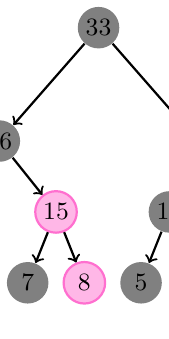
\begin{tikzpicture}[scale=1.8,auto,swap]
            \node[vertex] (0) at (-0.8,0.2) {1};
            \onslide<-1>{\node[vertex] (1) at (-0.4,0.2) {0};}
            \onslide<2->{\node[selected vertex] (1) at (-0.4,0.2) {0};}
            \node[vertex] (2) at (0.0,0.2) {7};
            \onslide<-1>{\node[vertex] (3) at (0.4,0.2) {8};}
            \onslide<2->{\node[selected vertex] (3) at (0.4,0.2) {8};}
            \node[vertex] (4) at (0.8,0.2) {5};
            \onslide<-1>{\node[vertex] (5) at (1.2,0.2) {9};}
            \onslide<2->{\node[selected vertex] (5) at (1.2,0.2) {9};}
            \onslide<-1>{\node[vertex] (6) at (1.6,0.2) {3};}
            \onslide<2->{\node[selected vertex] (6) at (1.6,0.2) {3};}

            \node[vertex] (7) at (-0.6,0.7) {1};
            \onslide<-1>{\node[vertex] (8) at (0.2,0.7) {15};}
            \onslide<2->{\node[selected vertex] (8) at (0.2,0.7) {15};}
            \node[vertex] (9) at (1.0,0.7) {14};

            \node[vertex] (10) at (-0.2,1.2) {16};
            \onslide<-1>{\node[vertex] (11) at (1.2,1.2) {17};}
            \onslide<2->{\node[selected vertex] (11) at (1.2,1.2) {17};}

            \node[vertex] (12) at (0.5,2.0) {33};

            \path[dedge] (7) -- (0);
            \path[dedge] (7) -- (1);
            \path[dedge] (8) -- (2);
            \path[dedge] (8) -- (3);
            \path[dedge] (9) -- (4);
            \path[dedge] (9) -- (5);

            \path[dedge] (10) -- (7);
            \path[dedge] (10) -- (8);
            \path[dedge] (11) -- (9);
            \path[dedge] (11) -- (6);

            \path[dedge] (12) -- (10);
            \path[dedge] (12) -- (11);

            \pgfresetboundingbox
            \path [use as bounding box] (0,0) rectangle (0.8,2.0);
        \end{tikzpicture}
    \end{figure}
    \bi
        \item For $sum$ some numbers are \textbf{redundant}\\
        \item For every node only the left successor is relevant
    \ei
\end{frame}


\begin{frame}[fragile]{Fenwick Trees}
    \bi
        \item Sum Segment Tree represented by an array of size $n$
        \item assume range is $1\dots n$
        \item use function $LSOne(x) = $\texttt{x\&(-x)} which returns the \textbf{value} of the least significant bit of $x$
	\bi
	  \item $LSOne(5) = 1$
	  \item $LSOne(12) = 4$
	  \item $LSOne(2n+1) = 1$
	  \item $LSOne(2^n) = 2^n$
	\ei
	\item construct $ft[x] = \sum_{i=x-LSOne(x)+1}^x A[i]$
    \ei
\end{frame}


\begin{frame}[fragile]{Fenwick Trees}
    $ft[x] = \sum_{i=x-LSOne(x)+1}^x A[i]$\\[\baselineskip]
    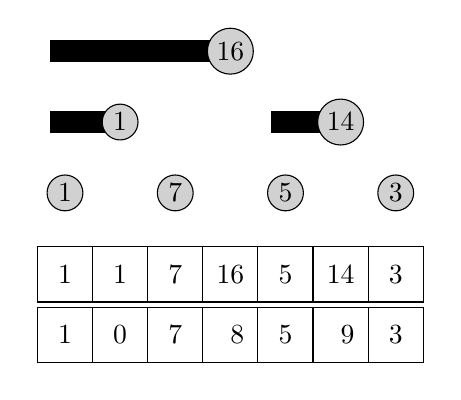
\begin{tikzpicture}[scale=1.8,auto,swap,
    array/.style={matrix of nodes,nodes={draw, minimum size=7mm, fill=white!30},column sep=-\pgflinewidth, row sep=0.5mm, nodes in empty cells,
% row 0/.style={nodes={draw=none, fill=none, minimum size=5mm}},
% row 1 column 1/.style={nodes={draw}}
    }]
      \matrix[array] (array) {
      1 & 1 & 7 & 16 & 5 & 14 & 3\\
      1 & 0 & 7 & \phantom{1}8 & 5 & \phantom{1}9 & 3\\ };
      %\node[draw, fill=gray, minimum size=4mm] at (array-2-2) (box) {};
      \node[draw, circle, fill=gray!30, inner sep=0.06cm, minimum size=1mm] at ($(array-2-1)+(0,1)$) (el1) {1};
      \node[draw, circle, fill=gray!30, inner sep=0.06cm, minimum size=1mm] at ($(array-2-2)+(0,1.5)$) (el2) {1};
      \node[draw, circle, fill=gray!30, inner sep=0.06cm, minimum size=1mm] at ($(array-2-3)+(0,1)$) (el3) {7};
      \node[draw, circle, fill=gray!30, inner sep=0.06cm, minimum size=1mm] at ($(array-2-4)+(0,2)$) (el4) {16};
      \node[draw, circle, fill=gray!30, inner sep=0.06cm, minimum size=1mm] at ($(array-2-5)+(0,1)$) (el5) {5};
      \node[draw, circle, fill=gray!30, inner sep=0.06cm, minimum size=1mm] at ($(array-2-6)+(0,1.5)$) (el6) {14};
      \node[draw, circle, fill=gray!30, inner sep=0.06cm, minimum size=1mm] at ($(array-2-7)+(0,1)$) (el7) {3};

      \begin{pgfonlayer}{bg}
	  \draw[fill=black] ($(el1) + (-0.1,0.575)$) rectangle ($(el2) - (0,0.075)$);
	  \draw[fill=black] ($(el1) + (-0.1,1.075)$) rectangle ($(el4) - (0,0.075)$);
	  \draw[fill=black] ($(el5) + (-0.1,0.575)$) rectangle ($(el6) - (0,0.075)$);
      \end{pgfonlayer}
    \end{tikzpicture}
\end{frame}


\begin{frame}[fragile]{Querying Fenwick Trees}
    $ft[x] = \sum_{i=x-LSOne(x)+1}^x A[i]$\\[\baselineskip]
    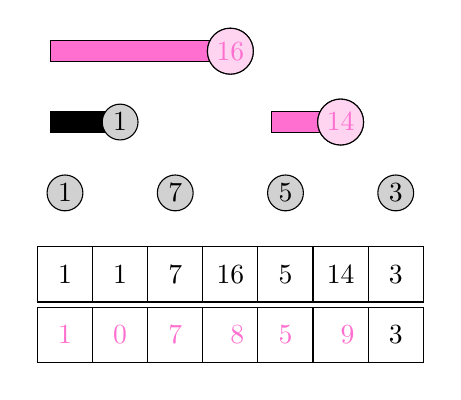
\begin{tikzpicture}[scale=1.8,auto,swap,
    array/.style={matrix of nodes,nodes={draw, minimum size=7mm, fill=white!30},column sep=-\pgflinewidth, row sep=0.5mm, nodes in empty cells,
% row 0/.style={nodes={draw=none, fill=none, minimum size=5mm}},
% row 1 column 1/.style={nodes={draw}}
    }]
      \matrix[array] (array) {
      1 & 1 & 7 & 16 & 5 & 14 & 3\\
      \textcolor{vhilight} 1 & \textcolor{vhilight}0 & \textcolor{vhilight}7 & \phantom{1}\textcolor{vhilight}8 & \textcolor{vhilight}5 & \phantom{1}\textcolor{vhilight}9 & 3\\ };
      %\node[draw, fill=gray, minimum size=4mm] at (array-2-2) (box) {};
      \node[draw, circle, fill=gray!30, inner sep=0.06cm, minimum size=1mm] at ($(array-2-1)+(0,1)$) (el1) {1};
      \node[draw, circle, fill=gray!30, inner sep=0.06cm, minimum size=1mm] at ($(array-2-2)+(0,1.5)$) (el2) {1};
      \node[draw, circle, fill=gray!30, inner sep=0.06cm, minimum size=1mm] at ($(array-2-3)+(0,1)$) (el3) {7};
      \onslide<-2>{\node[draw, circle, fill=gray!30, inner sep=0.06cm, minimum size=1mm] at ($(array-2-4)+(0,2)$) (el4) {16};}
      \onslide<3->{\node[draw, circle, fill=vhilight!30, inner sep=0.06cm, minimum size=1mm] at ($(array-2-4)+(0,2)$) (el4) {\textcolor{vhilight}{16}};}
      \node[draw, circle, fill=gray!30, inner sep=0.06cm, minimum size=1mm] at ($(array-2-5)+(0,1)$) (el5) {5};
      \onslide<-1>{\node[draw, circle, fill=gray!30, inner sep=0.06cm, minimum size=1mm] at ($(array-2-6)+(0,1.5)$) (el6) {14};}
      \onslide<2->{\node[draw, circle, fill=vhilight!30, inner sep=0.06cm, minimum size=1mm] at ($(array-2-6)+(0,1.5)$) (el6) {\textcolor{vhilight}{14}};}
      \node[draw, circle, fill=gray!30, inner sep=0.06cm, minimum size=1mm] at ($(array-2-7)+(0,1)$) (el7) {3};

      \begin{pgfonlayer}{bg}
	  \draw[fill=black] ($(el1) + (-0.1,0.575)$) rectangle ($(el2) - (0,0.075)$);
	  \onslide<-2>{\draw[fill=black] ($(el1) + (-0.1,1.075)$) rectangle ($(el4) - (0,0.075)$);}
	  \onslide<3->{\draw[fill=vhilight] ($(el1) + (-0.1,1.075)$) rectangle ($(el4) - (0,0.075)$);}
	  \onslide<-1>{\draw[fill=black] ($(el5) + (-0.1,0.575)$) rectangle ($(el6) - (0,0.075)$);}
	  \onslide<2->{\draw[fill=vhilight] ($(el5) + (-0.1,0.575)$) rectangle ($(el6) - (0,0.075)$);}
      \end{pgfonlayer}
    \end{tikzpicture}
    \bi
      \item $\mathrm{sum}(6) = $ \onslide<2->{\texttt{ft[4]}} \onslide<3->{$+$ \texttt{ft[6]}}
      \item<4-> $\mathrm{sum}(x) = ft[x] + \mathrm{sum}(x - LSOne(x))$ 
      \item<4-> $\mathrm{sum}(0) = 0$ 
    \ei
\end{frame}

\begin{frame}[fragile]{Updating Fenwick Trees}
    $ft[x] = \sum_{i=x-LSOne(x)+1}^x A[i]$\\[\baselineskip]
    \begin{tikzpicture}[scale=1.8,auto,swap,
    array/.style={matrix of nodes,nodes={draw, minimum size=7mm, fill=white!30},column sep=-\pgflinewidth, row sep=0.5mm, nodes in empty cells,
% row 0/.style={nodes={draw=none, fill=none, minimum size=5mm}},
% row 1 column 1/.style={nodes={draw}}
    }]
      \matrix[array] (array) {
      1 & 1 & 7 & 16 & 5 & 14 & 3\\
      \textcolor{vhilight} 1 & \textcolor{vhilight}0 & \only<1>{\textcolor{vhilight}7}\only<2->{\textcolor{vhilight}5} & \phantom{1}\textcolor{vhilight}8 & \textcolor{vhilight}5 & \phantom{1}\textcolor{vhilight}9 & 3\\ };
      %\node[draw, fill=gray, minimum size=4mm] at (array-2-2) (box) {};
      \node[draw, circle, fill=gray!30, inner sep=0.06cm, minimum size=1mm] at ($(array-2-1)+(0,1)$) (el1) {1};
      \node[draw, circle, fill=gray!30, inner sep=0.06cm, minimum size=1mm] at ($(array-2-2)+(0,1.5)$) (el2) {1};
      \onslide<-2>{\node[draw, circle, fill=gray!30, inner sep=0.06cm, minimum size=1mm] at ($(array-2-3)+(0,1)$) (el3) {7};}
      \onslide<3->{\node[draw, circle, fill=vhilight!30, inner sep=0.06cm, minimum size=1mm] at ($(array-2-3)+(0,1)$) (el3) {\textcolor{vhilight}5};}
      \onslide<-3>{\node[draw, circle, fill=gray!30, inner sep=0.06cm, minimum size=1mm] at ($(array-2-4)+(0,2)$) (el4) {16};}
      \onslide<4->{\node[draw, circle, fill=vhilight!30, inner sep=0.06cm, minimum size=1mm] at ($(array-2-4)+(0,2)$) (el4) {\textcolor{vhilight}{14}};}
      \node[draw, circle, fill=gray!30, inner sep=0.06cm, minimum size=1mm] at ($(array-2-5)+(0,1)$) (el5) {5};
      \node[draw, circle, fill=gray!30, inner sep=0.06cm, minimum size=1mm] at ($(array-2-6)+(0,1.5)$) (el6) {14};
      \node[draw, circle, fill=gray!30, inner sep=0.06cm, minimum size=1mm] at ($(array-2-7)+(0,1)$) (el7) {3};

      \begin{pgfonlayer}{bg}
	  \draw[fill=black] ($(el1) + (-0.1,0.575)$) rectangle ($(el2) - (0,0.075)$);
	  \draw[fill=black] ($(el1) + (-0.1,1.075)$) rectangle ($(el4) - (0,0.075)$);
	  \draw[fill=black] ($(el5) + (-0.1,0.575)$) rectangle ($(el6) - (0,0.075)$);
      \end{pgfonlayer}
    \end{tikzpicture}
    \bi
      \item $\mathrm{add}(3,-2)$
    \ei
\end{frame}

\begin{frame}[fragile]{Fenwick Trees - Code}
%     \vspace{-20pt}
    \begin{minted}[fontsize=\scriptsize]{cpp}
int fwt_size, bi_tree[MAXN];

void clear(int size) {
    memset(bi_tree, 0, sizeof(int) * size); fwt_size = size;
}
void add(int pos, int val) {
    if (!pos) {
        bi_tree[0] = bi_tree[0] + val;
        return;
    }
    while (pos < fwt_size) {
        bi_tree[pos] = bi_tree[pos] + val;
        pos += pos & (-pos);
    }
}
int rank(int pos) {
    if (pos < 0) return 0;
    int res = bi_tree[0];
    while (pos) {
        res = res + bi_tree[pos];
        pos &= pos - 1;
    }
    return res;
}
    \end{minted}
\end{frame}

\begin{frame}{Fenwick Trees}
    \bi
        \item Lightweight implementation of Sum Segment Tree
        \bi
	  \item build a Fenwick Tree\onslide<2->{ in {\color{hilight}{$O(n)$}}}
	  \item query a range\onslide<3->{ in {\color{hilight}{$O(\log n)$}}}
	  \item update a single value\onslide<4->{ in {\color{hilight}{$O(\log n)$}}}
	\ei
    \ei
\end{frame}

\end{document}
